% Scene + reversed-triangle camera (apex back, screen front) + black ray + flat-grey surfel.
\documentclass[tikz,border=4pt]{standalone}
\usepackage{tikz}
\usepackage{amsmath}
\usepackage{amssymb}
\usepackage{xcolor}
\usetikzlibrary{positioning, calc, arrows.meta, shapes.geometric}

\begin{document}
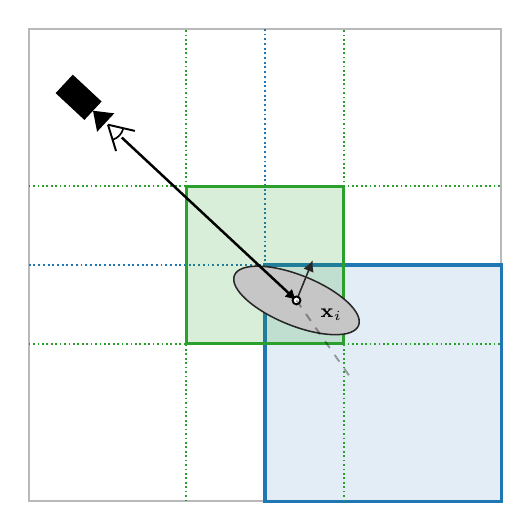
\begin{tikzpicture}[
  font=\sffamily\footnotesize,
  >={Latex[length=4pt,width=4pt]},
]
% ---------------- scene bbox ----------------
\draw[gray!55, thick] (0,0) rectangle (6,6);

% =====================================================================
% 2x2 coarse grid (BLUE) — bottom-right cell highlighted
% =====================================================================
\definecolor{cgridA}{HTML}{1F77B4}
\draw[cgridA, densely dotted, line width=0.7pt] (3,0) -- (3,6);
\draw[cgridA, densely dotted, line width=0.7pt] (0,3) -- (6,3);
\fill[cgridA, opacity=0.13] (3,0) rectangle (6,3);
\draw[cgridA, line width=1.1pt] (3,0) rectangle (6,3);

% =====================================================================
% 3x3 finer grid (GREEN) — middle cell highlighted
% =====================================================================
\definecolor{cgridB}{HTML}{2CA02C}
\foreach \x in {2,4} {
  \draw[cgridB, densely dotted, line width=0.6pt] (\x,0) -- (\x,6);
}
\foreach \y in {2,4} {
  \draw[cgridB, densely dotted, line width=0.6pt] (0,\y) -- (6,\y);
}
\fill[cgridB, opacity=0.18] (2,2) rectangle (4,4);
\draw[cgridB, line width=1.1pt] (2,2) rectangle (4,4);

% =====================================================================
% Surfel + intersection (target)
% =====================================================================
\coordinate (xint) at (3.4, 2.55);
\begin{scope}[shift={(3.4,2.55)}, rotate=-22]
  \filldraw[gray!45, draw=gray!30!black, line width=0.55pt]
            (0,0) ellipse [x radius=0.85, y radius=0.32];
  \draw[->, gray!30!black, line width=0.55pt] (0,0) -- (0,0.55);
\end{scope}

% =====================================================================
% Camera glyph (new style): body + reverse-tip triangle + FOV with arc.
% Oriented along the viewing direction toward x_i.
% =====================================================================
\pgfmathsetmacro{\apexx}{0.45}
\pgfmathsetmacro{\apexy}{5.30}
\pgfmathsetmacro{\dxx}{3.4}
\pgfmathsetmacro{\dyy}{2.55}
\pgfmathsetmacro{\vx}{\dxx - \apexx}
\pgfmathsetmacro{\vy}{\dyy - \apexy}
\pgfmathsetmacro{\vlen}{sqrt(\vx*\vx + \vy*\vy)}
\pgfmathsetmacro{\ux}{\vx / \vlen}
\pgfmathsetmacro{\uy}{\vy / \vlen}
\pgfmathsetmacro{\camRot}{atan2(\uy, \ux)}

\pgfmathsetmacro{\sicbw}{0.50}
\pgfmathsetmacro{\sicbh}{0.32}
\pgfmathsetmacro{\sictlen}{0.22}
\pgfmathsetmacro{\sicgap}{0.04}
\pgfmathsetmacro{\sicangDeg}{30}
\pgfmathsetmacro{\sicarmLen}{0.35}
\pgfmathsetmacro{\sicarcR}{0.20}
\pgfmathsetmacro{\sicarmX}{\sicarmLen*cos(\sicangDeg)}
\pgfmathsetmacro{\sicarmY}{\sicarmLen*sin(\sicangDeg)}
\pgfmathsetmacro{\sicFovApexX}{\sicbw + \sictlen + \sicgap}
\pgfmathsetmacro{\siccamOutX}{\sicFovApexX + \sicarcR + 0.04}

\pgfmathsetmacro{\rayWX}{\apexx + \siccamOutX*\ux}
\pgfmathsetmacro{\rayWY}{\apexy + \siccamOutX*\uy}
\coordinate (rayStart) at (\rayWX, \rayWY);

% Ray from camera output toward x_i
\draw[black, line width=0.9pt, ->]
  (rayStart) -- (xint);

\begin{scope}[shift={(\apexx, \apexy)}, rotate=\camRot]
  \fill[black] (0, -\sicbh/2) rectangle (\sicbw, \sicbh/2);
  \fill[black] (\sicbw, 0) -- (\sicbw + \sictlen,  \sicbh/2)
                           -- (\sicbw + \sictlen, -\sicbh/2) -- cycle;
  \pgfmathsetmacro{\fovx}{\sicFovApexX}
  \draw[black, line width=0.7pt] (\fovx, 0) -- (\fovx + \sicarmX,  \sicarmY);
  \draw[black, line width=0.7pt] (\fovx, 0) -- (\fovx + \sicarmX, -\sicarmY);
  \draw[black, line width=0.6pt]
    (\fovx + \sicarcR, 0) arc (0:\sicangDeg:\sicarcR);
  \draw[black, line width=0.6pt]
    (\fovx + \sicarcR, 0) arc (0:-\sicangDeg:\sicarcR);
\end{scope}

\draw[black, line width=0.7pt, fill=white] (xint) circle (0.05);
\node[font=\sffamily\scriptsize, anchor=west]
  at ($(xint)+(0.18,-0.18)$) {$\mathbf{x}_i$};
% faint continuation past the disk
\draw[black, line width=0.7pt, dashed, opacity=0.35]
  (xint) -- ($(xint)+(0.7,-1.0)$);

\end{tikzpicture}
\end{document}
